\documentclass{beamer}

%%%%%%%%%%%%
% PACKAGES %
\usepackage{amsmath}
\usepackage{color}

%%%%%%%%%
% THEME %
\usetheme{Warsaw}
\setbeamertemplate{navigation symbols}{}

%%%%%%%%%%%%%%%%%%%
% CUSTOM COMMANDS %
\DeclareMathOperator{\Tr}{Tr}
	\DeclareMathOperator*{\Cov}{Cov}
	\DeclareMathOperator{\cov}{Cov}

	\newcommand{\ket}[1]{\ensuremath{\vert #1 \rangle}}
	\newcommand{\bra}[1]{\ensuremath{\langle #1 \vert}}
	\newcommand{\braket}[2]{\ensuremath{\langle #1 \vert #2 \rangle}}
	\newcommand{\braOket}[3]{\ensuremath{\langle #1 \vert #2 \vert #3 \rangle}}
	\newcommand{\ketbra}[2]{\ensuremath{\vert #1 \rangle \! \langle #2 \vert}}
	\newcommand{\expect}[1]{\ensuremath{\langle #1 \rangle}}
	\newcommand{\varian}[1]{\ensuremath{\left(\Delta #1 \right)^2}}
	\newcommand{\ver}[2]{\ensuremath{\genfrac{}{}{0pt}{}{#1}{#2}}}
	\newcommand{\tr}[1]{\ensuremath{\Tr \lcua #1\rcua}}
	\newcommand{\trsub}[2]{\ensuremath{\Tr_{#1} \lcua #2 \rcua }}
	\newcommand{\bsym}[1]{\ensuremath{\boldsymbol{#1}}}
	\newcommand{\citate}[1]{{\footnotesize{\color{gray}[ #1 ]}}

	}

	\def\be{\begin{equation}}
	\def\ee{\end{equation}}
	\def\bea{\begin{eqnarray}}
	\def\eea{\end{eqnarray}}
	\def\bse{\begin{subequations}}
	\def\ese{\end{subequations}}
	\def\mtxid{\mathbbm{1}}
	\def\lpar{\left(}
	\def\rpar{\right)}
	\def\lcua{\left[}
	\def\rcua{\right]}
	\def\lcor{\left\{}
	\def\rcor{\right\}}
	\def\lang{\left\langle}
	\def\rang{\right\rangle}
	\def\l{\left}
	\def\r{\right}
	\def\nnnl{\nonumber\\}
	\def\nnnlq{\nonumber\\ && \quad}
	\def\nnnlqq{\nonumber\\ && \qquad}
	\def\nnnlqqq{\nonumber\\ && \quad\qquad}
	\def\ie{, \textit{i.e.}, }
	\def\etal{\textit{et al. }}

%%%%%%%%%%%%%%%%
% THE DOCUMENT %
\begin{document}

%%%%%%%%%%%%%%
% TITLE PAGE %
\title{Optimal bound on the quantum\\ Fisher information}

	\subtitle{\it Based on few initial expectation values
	}

	\author[Iagoba, Matthias, Otfried, G\'eza]{
		\textbf{Iagoba Apellaniz} \inst{1},
		Matthias Kleinmann \inst{1},
		Otfried G\"uhne \inst{2},
		\& G\'eza T\'oth \inst{1,3,4}
	}
	\institute{
		\textbf{iagoba.apellaniz@gmail.com}\\
		\vspace{5px}
		\inst{1}
		Department of Theoretical Physics, University of the Basque Country, Spain\\
		\inst{2}
		Naturwissenschaftlich-Technische Fakult\"at, Universit\"at Siegen, Germany\\
		\inst{3}
		IKERBASQUE, Basque Foundation for Science, Spain\\
		\inst{4}
		Wigner Research Centre for Physics, Hungarian Academy of Sciences, Hungary
	}


	\date{Recent Advances in Quantum Metrology; Warsaw - 2016}


%%%%%%%%%%%%%%%%
% BEGIN FRAMES %
\begin{frame}
	\titlepage
\end{frame}

% Reset counter to skip title page
\addtocounter{framenumber}{-1}
	\addtobeamertemplate{navigation symbols}{}{%
    \usebeamerfont{footline}%
    \usebeamercolor[fg]{footline}%
    \hspace{1em}%
    {\small\insertframenumber}
		\vspace{2px}
	}

\begin{frame}
	\frametitle{Outline}
	\tableofcontents
\end{frame}

\section{Introduction and Motivation}

	\begin{frame}
		\begin{itemize}
			\item<1-> \emph{\color{blue} Many \bf inequalities} have been proposed to lower bound the quantum Fisher Information.
		  	\only<1>{
					\begin{block}{Bounds for qFI}
						\vspace{4px}
							\small
							\[F_Q[\varrho,J_z]\geq 	\frac{\expect{J_x}^2}{\varian{J_y}},
								\qquad\quad
								F_Q[\varrho,J_y]\geq \beta^{-2}\frac{\expect{J_x^2+J_z^2}}{\varian{J_z}+\frac{1}{4}},
							\]
							\[F_Q[\varrho,J_z]\geq \frac{4(\expect{J_x^2+J_y^2})^2} {2\sqrt{\varian{J_x^2}\varian{J_y^2}} +\expect{J_x^2} -2\expect{J_y^2}(1+\expect{J_x^2}) +6\expect{J_yJ_x^2J_y} }
							\]
							\vspace{-4px}
					\end{block}
					\citate{L. Pezz\'e \& A. Smerzi, PRL \textbf{102}, 100401 (2009)}
					\citate{Z. Zhang \& L.-M. Duan, NJP \textbf{16}, 103037 (2014)}
					\citate{\textbf{I.A.}, B. L\"ucke, J. Peise, C. Klempt \& G. Toth, NJP \textbf{17}, 083027 (2015)}

				}
			\only<2->{
			\vspace{10px}
			\item For large systems, we only have \emph{\color{blue} a couple of expectation values} to characterise the state.
				\only<2,3>{
				\begin{figure}
  				\includegraphics<2>[height=107px]{img/ghz3-histogram.pdf}
					\includegraphics<3>[height=107px]{img/ghz3-histogram-banned.pdf}
				\end{figure}}
			}
			\only<4->{
			\vspace{10px}
			\item	The archetypical criteria that shows \emph{\color{blue}metrologically useful entanglement}.
				\only<4>{
					\[ F_Q[\varrho,J_z]\geq 	\frac{\expect{J_x}}{\varian{J_z}} \]
					\citate{L. Pezz\'e \& A. Smerzi, PRL \textbf{102}, 100401 (2009)}
					\vspace{22px}
				}
				\vspace{5px}
			}
			\only<5>{
			\vspace{10px}
			\item It is essential either to \emph{\color{blue} verify them or find new ones} for different set of expectation values.
			\vspace{27px}
			}
		\end{itemize}
	\end{frame}

\section[QFI based on expectation values]{QFI based on expectation values: Are they optimal?}

	\begin{frame}
		\tableofcontents[currentsection]

	\end{frame}

	\begin{frame}
		\frametitle{The non-trivial exercise of computing the qFI}

		\begin{itemize}
			\item<1-> Different forms of the qFI
				\begin{block}
					{}
					\small
					\[
						F_Q[\varrho,J_z]=2 \sum_{\lambda,\gamma} \frac{(p_\lambda-p_\gamma)^2}{p_\lambda+p_\gamma} |\braOket{\lambda}{J_z}{\gamma}|^2
					\]
					\hspace{10px}Alternatively, as convex roof
					\[
					  F_Q[\varrho,J_z]=\min_{\{p_k,\ket{\Psi_k}\}} 4\sum_k p_k \varian{J_z}_{\ket{\Psi_k}}
					\]
				\end{block}
				\citate{M.G.A. Paris, Int. J. Quant. Inf. \textbf{7}, 125 (2009)}
				\citate{G. T\'oth \& D. Petz, PRA \textbf{87}, 032324 (2013)}
				\citate{S. Yu, arXiv:1302.5311}
				\vspace{2px}

			\item<2-> For pure states it's extremely simple
				{\small
				\[
					F_Q[\varrho,J_z] = 4\varian{J_z}
				\]
				}

		\end{itemize}

	\end{frame}

	\subsection{Optimisation problem}

		\begin{frame}
			\frametitle{Optimisation based on the Legendre Transform}
			\begin{itemize}
				\item When $g(\varrho)$ is a \emph{\color{blue} convex roof}
					\begin{block}
						{}
						{\small
						\vspace{8px}
						\[
						g(\varrho)\geq\mathcal{B}(w:=\tr{\varrho W}) = \sup_{r} \big( r w - \sup_{\ket{\psi}} [ r\expect{W} - g(\ket{\psi}) ] \big).
						\]}
					\end{block}
			\end{itemize}

			\citate{O. G\"uhne, M. Reimpell \& R.F. Werner, PRL \textbf{98}, 110502 (2007)}
			\citate{J. Eisert, F.G.S.L. Brand\~ao \& K.M.R. Audenaert, NJP \textbf{9}, 46 (2007)}
		\end{frame}

		\begin{frame}
			\begin{block}
				{Optimisation for the qFI}
				\vspace{4px}
				\hspace{10px}The \emph{\color{blue} simplicity} of qFI for pure states leads to
				{\small
				\[
				\mathcal{F}(w) = \sup_{r} \big( r w - {\color{blue}\sup_{\mu} [ \lambda_{\max} ( r W - 4(J_z-{\color{blue}\mu})^2 ) ]} \big).
				\]}

				\hspace{10px}For more parameters
				{\small
				\[
				\mathcal{F}(\mathbf{w}) = \sup_{\mathbf{r}} \big( \mathbf{r}\cdot \mathbf{w} - {\color{blue}\sup_{\mu} [ \lambda_{\max} ( \mathbf{r}\cdot \mathbf{W} - 4(J_z-{\color{blue}\mu})^2 ) ]} \big).
				\]}
				\vspace{-4px}
			\end{block}

			\citate{\textbf{I.A.}, M. Kleinmann, O. G\"uhne \& G. T\'oth, arXiv:1511.05203}

		\end{frame}

\section{Case study}

		\begin{frame}
			\tableofcontents[currentsection]

		\end{frame}

	\subsection{Fidelities}

		\begin{frame}
			\begin{itemize}
				\item<1-> Measuring $F_{\rm GHZ}$ and $F_{\rm Dicke}$
				\vspace{10px}

				\onslide<2->{
				\begin{figure}
					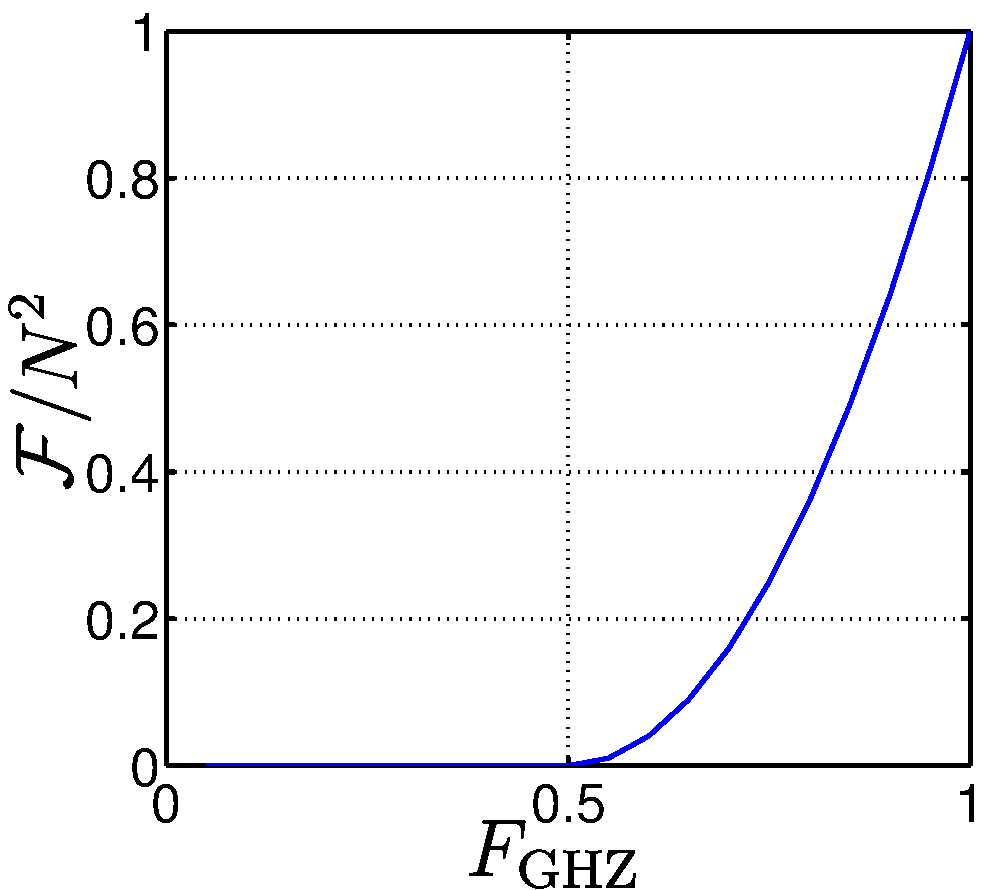
\includegraphics[height=110px]{img/lb-ghzfidelity.pdf}
					\hspace{20px}
					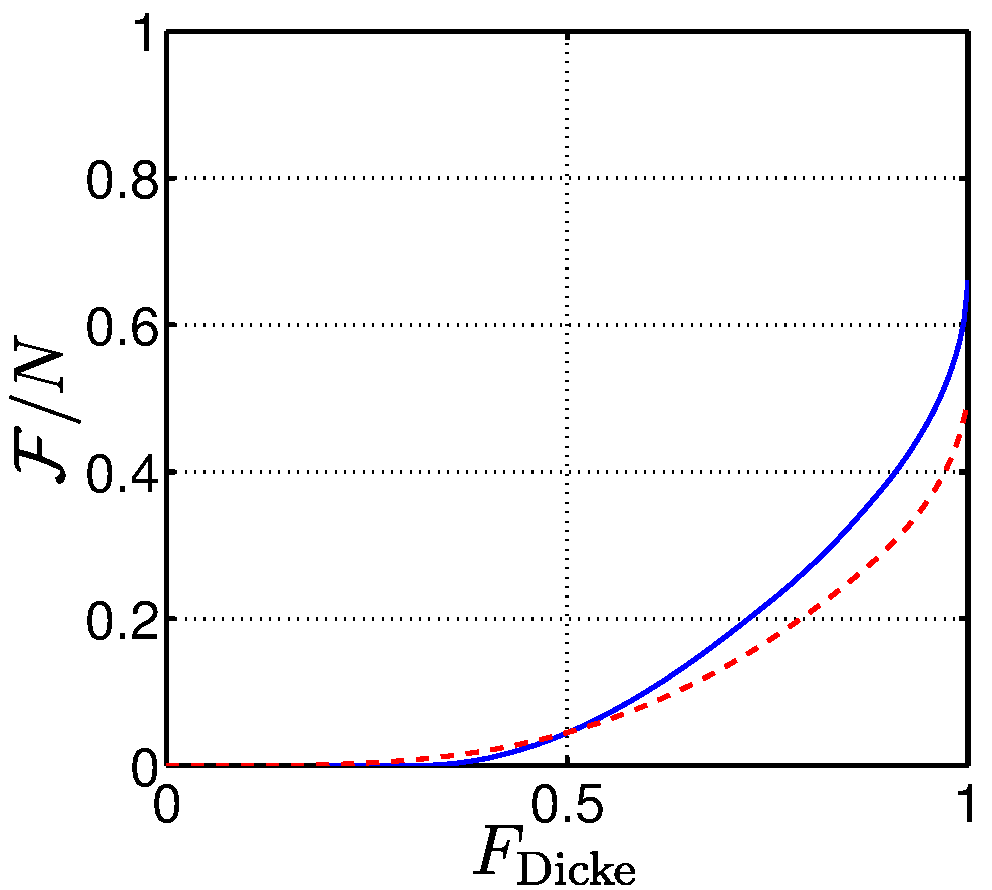
\includegraphics[height=110px]{img/lb-dickefidelity}
				\end{figure}
				\vspace{-10px}
				}
				\item<3-> For fidelity of GHZ $\implies$ \emph{\color{blue}analytic soulution}
			\end{itemize}
			\onslide<3>{\begin{block}
				{}
				\[
				\mathcal{F}=\Theta(F_{\rm GHZ}-0.5)(2F_{\rm GHZ}-1)^2 N^2
				\]
				\vspace{-12px}
			\end{block}}
		\end{frame}

	\subsection{Spin-squeezed states}

		\begin{frame}

			\frametitle{Measuring $\expect{J_z}$ and $\varian{J_x}$ for Spin Squeezed States}

			\begin{itemize}
				\item<1-> 3 operators {\color{blue}$\{ J_z,J_x,J_x^2 \}$}
				\vspace{5px}
				\item<2-> Reducing one dimension of $\mathcal{F}$ on the $\expect{J_x}$ direction
				\begin{block}{}
					\[\mathcal{F} \geq \mathcal{F}(\expect{J_x}=0)\]
					\[\Downarrow\]
					\[\mathcal{F}(\expect{J_z},{\color{blue}\varian{J_x}}) := \mathcal{F}(\expect{J_z},{\color{blue}\expect{J_x^2}})
					\]
					\vspace{-12px}
				\end{block}
				\vspace{5px}
				\item<3-> Pezze-Smerzi bound, $F_Q\geq \expect{J_z}^2/\varian{J_x}$, can be verified.
			\end{itemize}

		\end{frame}

		\begin{frame}
			\begin{itemize}
				\item 4-particle system
			\end{itemize}
			\begin{figure}
				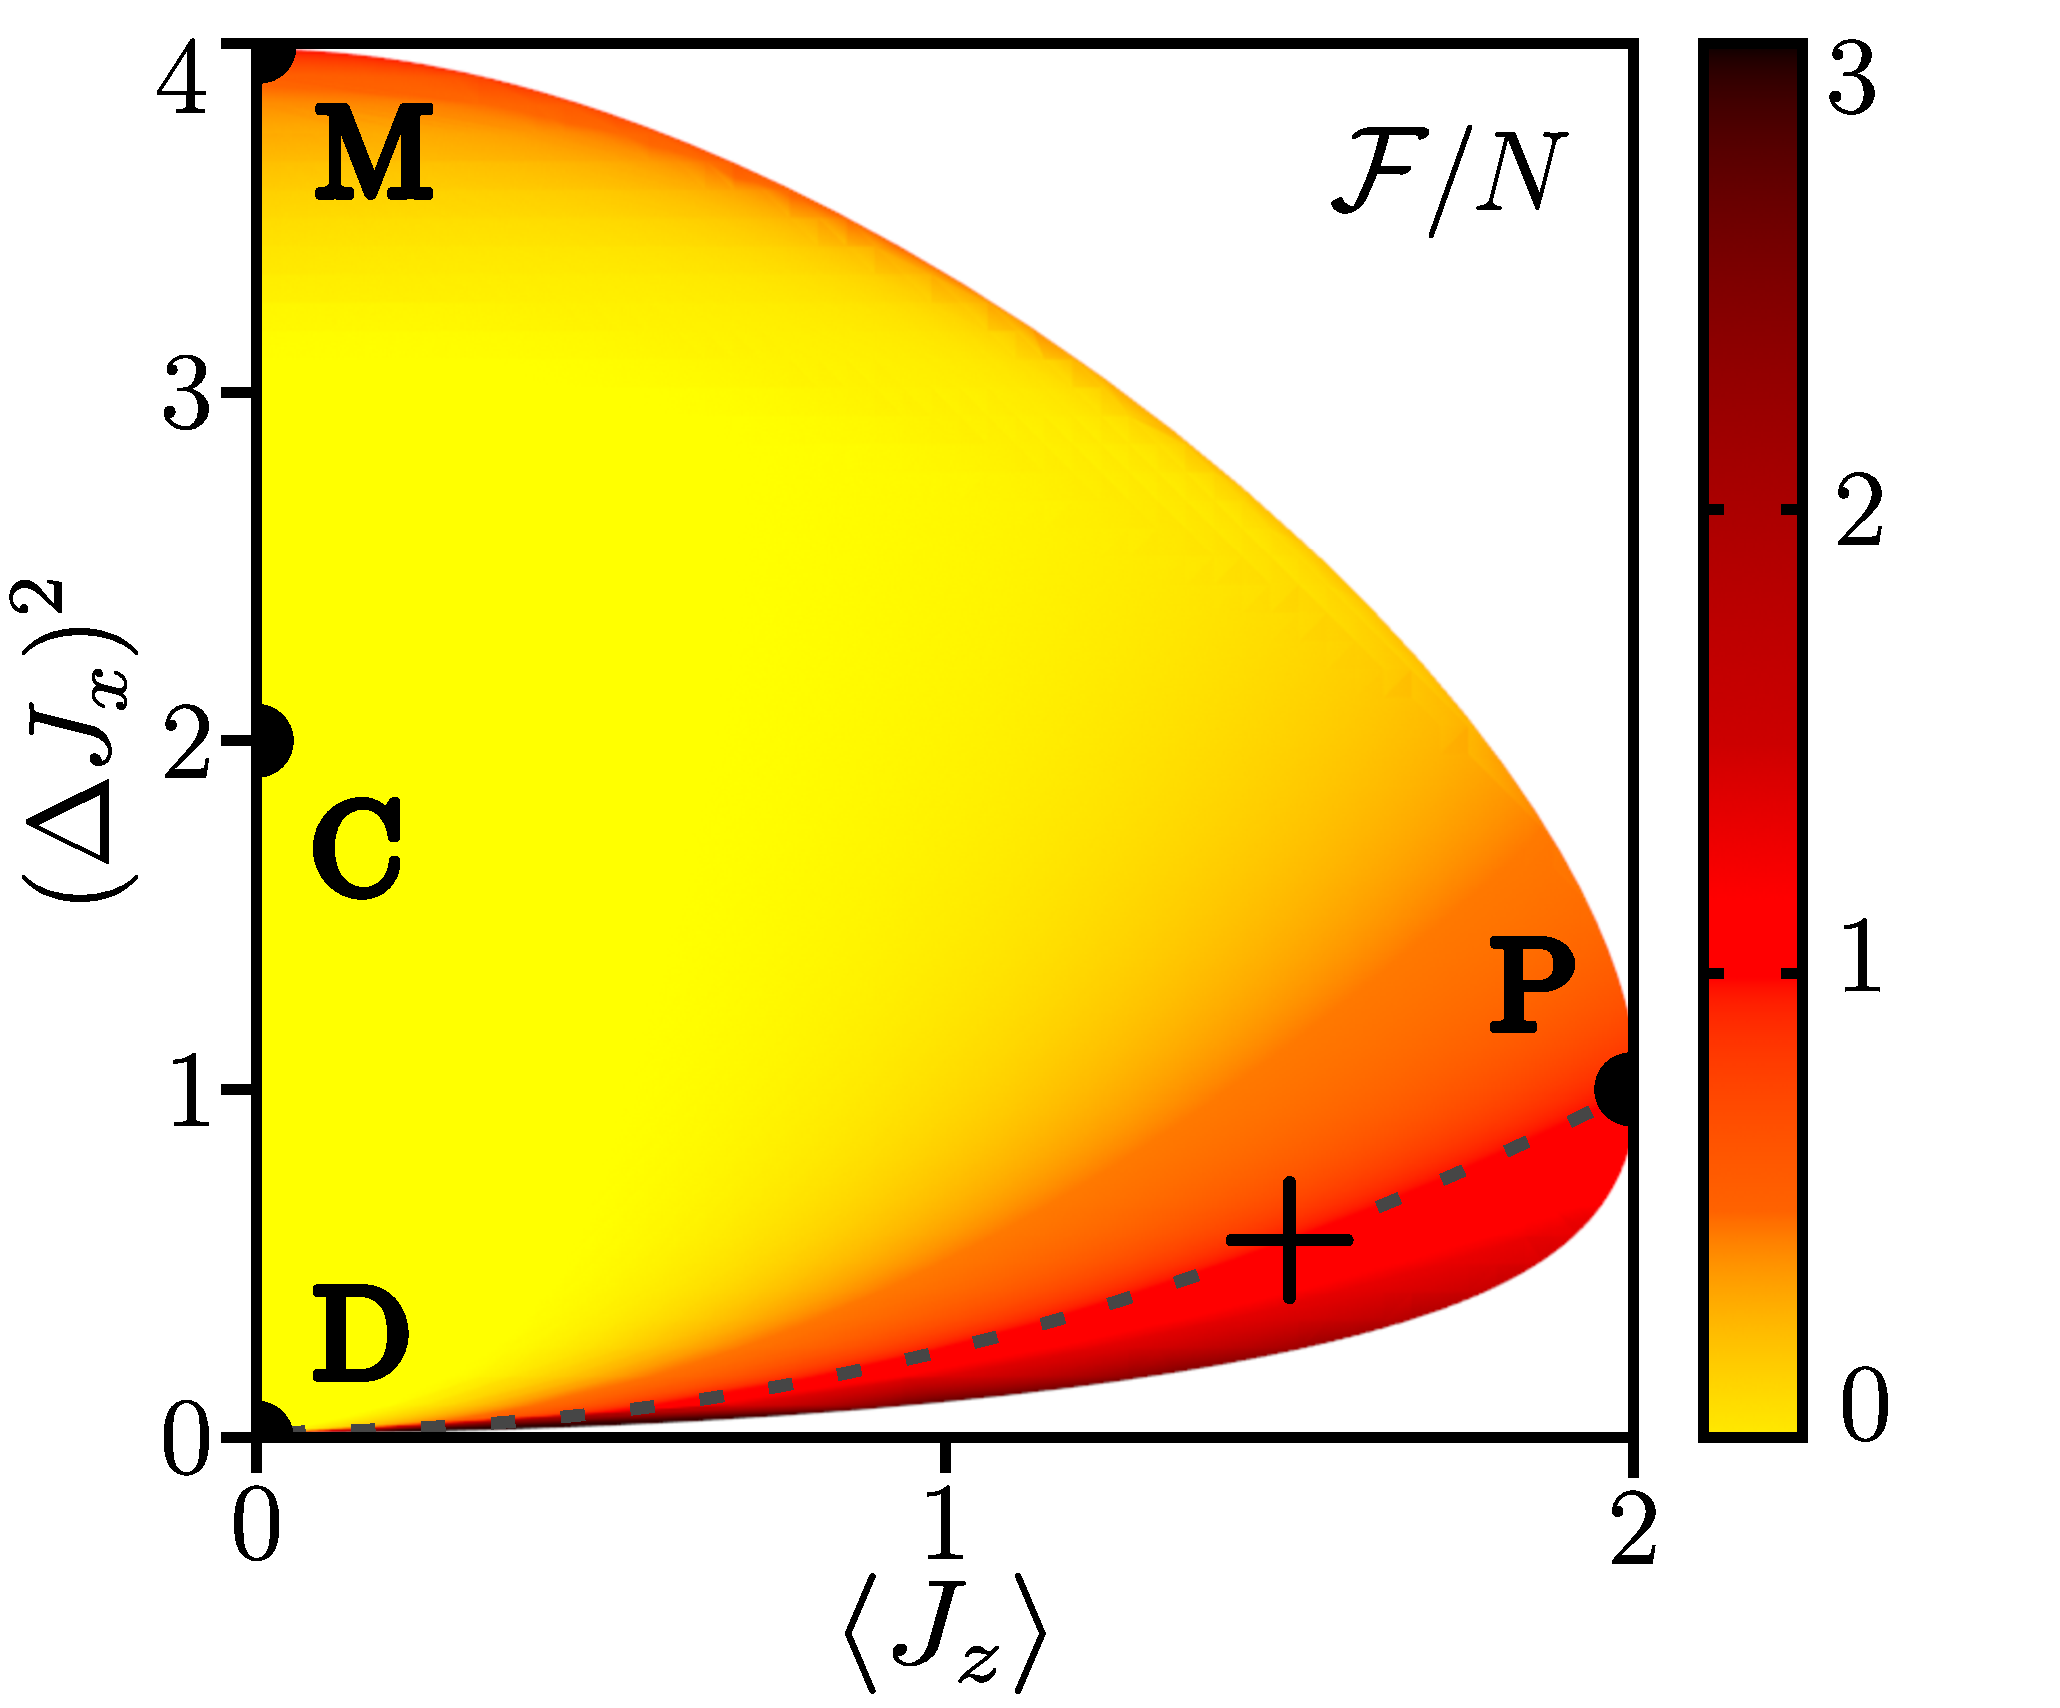
\includegraphics[height=120px]{img/lb-spsq.pdf}
				\hspace{15px}
				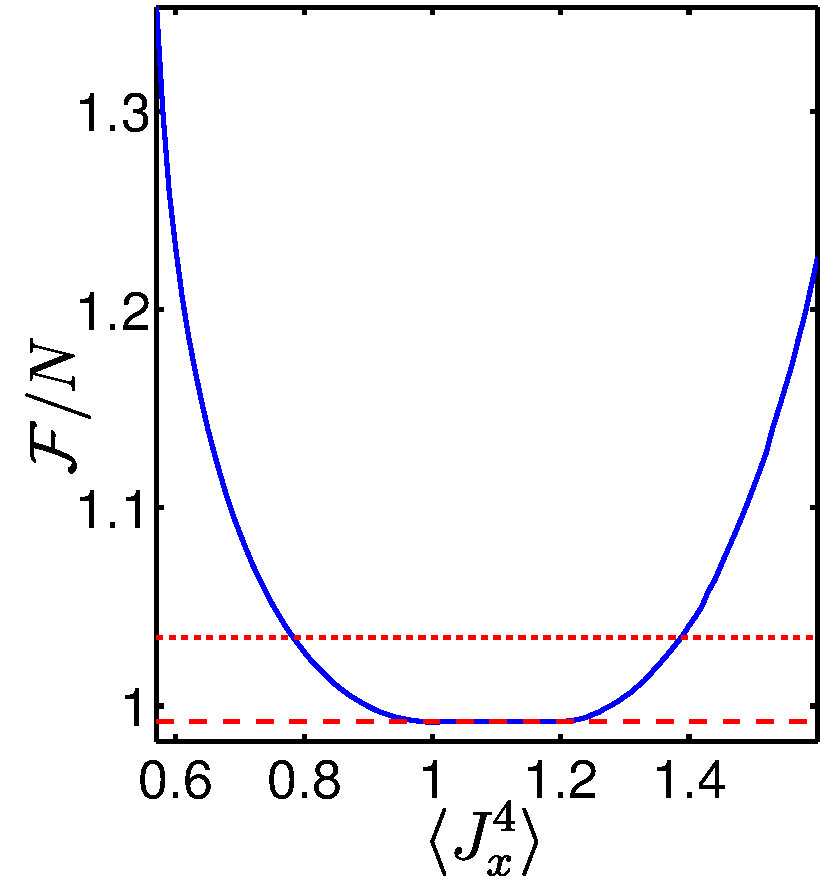
\includegraphics[height=120px]{img/4thparameter-spsq.pdf}
			\end{figure}
			For $\varian{J_x}<1.5$ it almost coincides with the P-S bound $F_Q\geq \expect{J_z}^2/\varian{J_x}$.

			\citate{\textbf{I.A.}, M. Kleinmann, O. G\"une \& G. T\'oth, arXiv:1511.05203}

		\end{frame}

		\begin{frame}
			\frametitle{Scaling the result for large systems}

			{\small Experimental setup $\rightarrow$ \citate{C. Gross {\it et al.}, Nature {\bf 464}, 1165 (2010)}}
				\begin{block}
					{}
					\[
					N = {\color{red}2300}\qquad \xi^2_{\rm s} =-8.2{\rm dB}=0.1514
					\]
					\vspace{-12px}
				\end{block}
				\begin{itemize}
					\item<2-> We choose
					\[ \expect{J_z} = 0.85 \frac{N}{2}
					\]
					\item<3-> P-S bound results is
					\[
					\frac{F_Q}{N} \geq \frac{1}{\xi_{\rm s}^2} = 6.605
					\]
				\end{itemize}
		\end{frame}

		\begin{frame}

			\begin{itemize}
				\item Starting from small systems.
				\vspace{5px}
				\item The results with our method converge to P-S bound!
			\end{itemize}
			\begin{figure}
				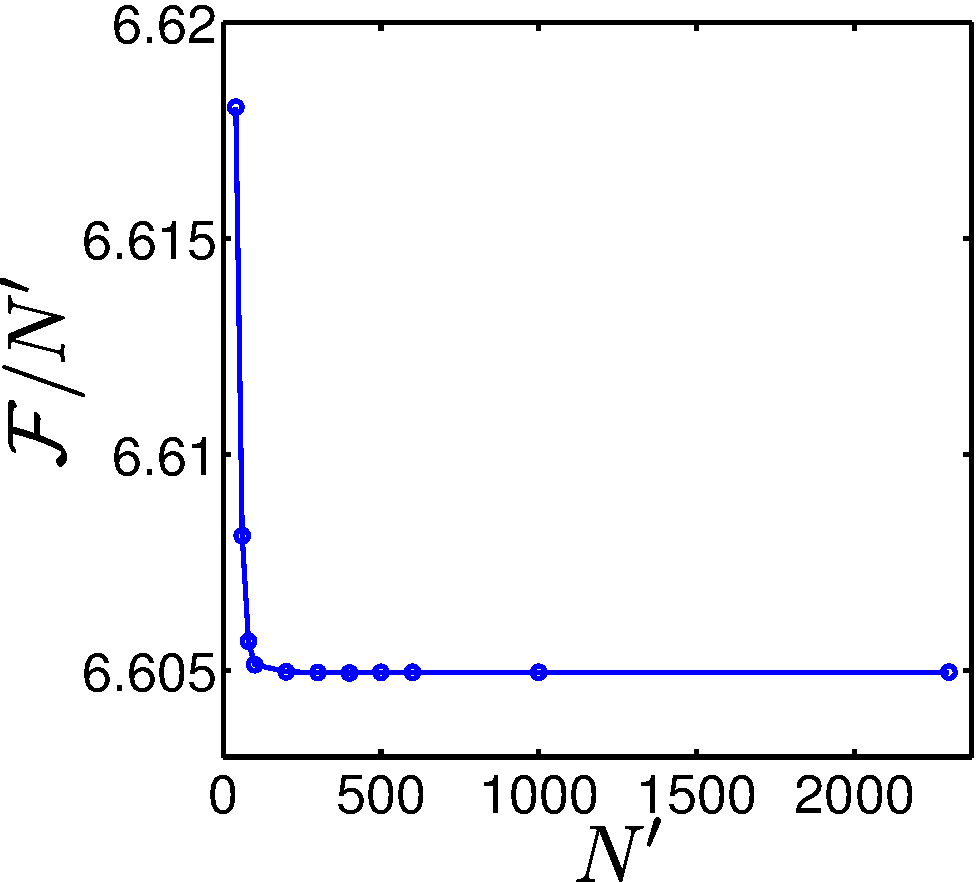
\includegraphics[height=130px]{img/scaling-spsq.pdf}
			\end{figure}

		\end{frame}

	\subsection{Unpolarised Dicke states}

		\begin{frame}
			\frametitle{Metrology with unpolarised Dicke states}
			\begin{itemize}
				\item<1-> 3 operators $\color{blue}\{J_x^2,J_y^2,J_z^2\}$; Constraint: $\expect{J_x^2}=\expect{J_y^2}$.
				\vspace{5px}
				\item<2-> For $\sum_l \expect{J_l^2} = \tfrac{N}{2} (\tfrac{N}{2}+1)$ and 6 particles:
				\begin{figure}
					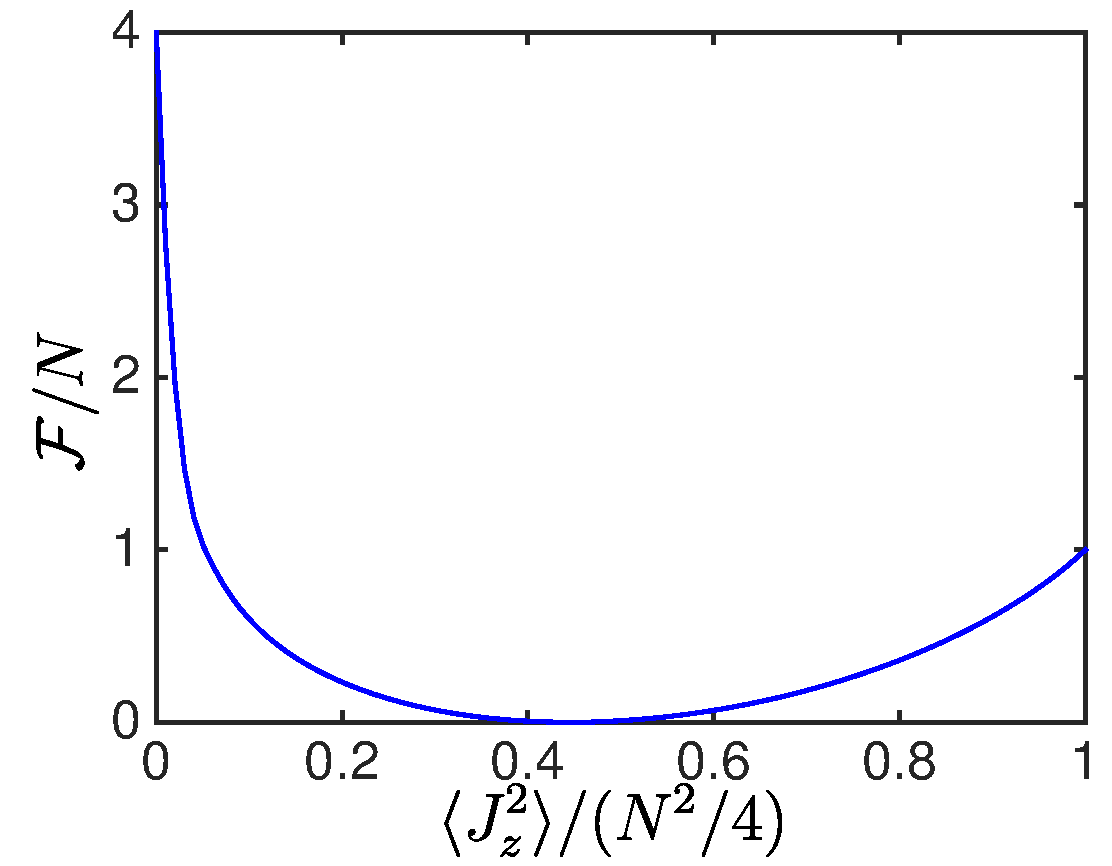
\includegraphics[height=120px]{img/upperboundary-dicke.pdf}
				\end{figure}

			\end{itemize}

		\end{frame}

		\begin{frame}
			\frametitle{Realistic characterisation of Dicke state}
			{\small Experiment $\rightarrow$}
			\citate{B. L\"ucke {\it et al.}, PRL \textbf{112}, 155304 (2014)}

				\begin{block}{}
					\vspace{-1px}
					\bea
					 	&N ={\color{red} 7900} \hspace{60px} \expect{J_z^2}=112\pm 31 &
						\nnnl\nnnl
						&\expect{J_x^2}=\expect{J_y^2}  =  6 \times 10^6 \pm 0.6\times 10^6 &\nnnl
						\nonumber
					\eea
				\end{block}

			\begin{itemize}
				\item For that large system we use \emph{\color{blue} extrapolation methods} similar to spin-squeezed states.
			\end{itemize}
		\end{frame}

		\begin{frame}
			\begin{itemize}
				\item We obtain a numerical lower bound for this \emph{\color{blue}large system}.
			\end{itemize}
			\vspace{-10px}
			\begin{figure}
				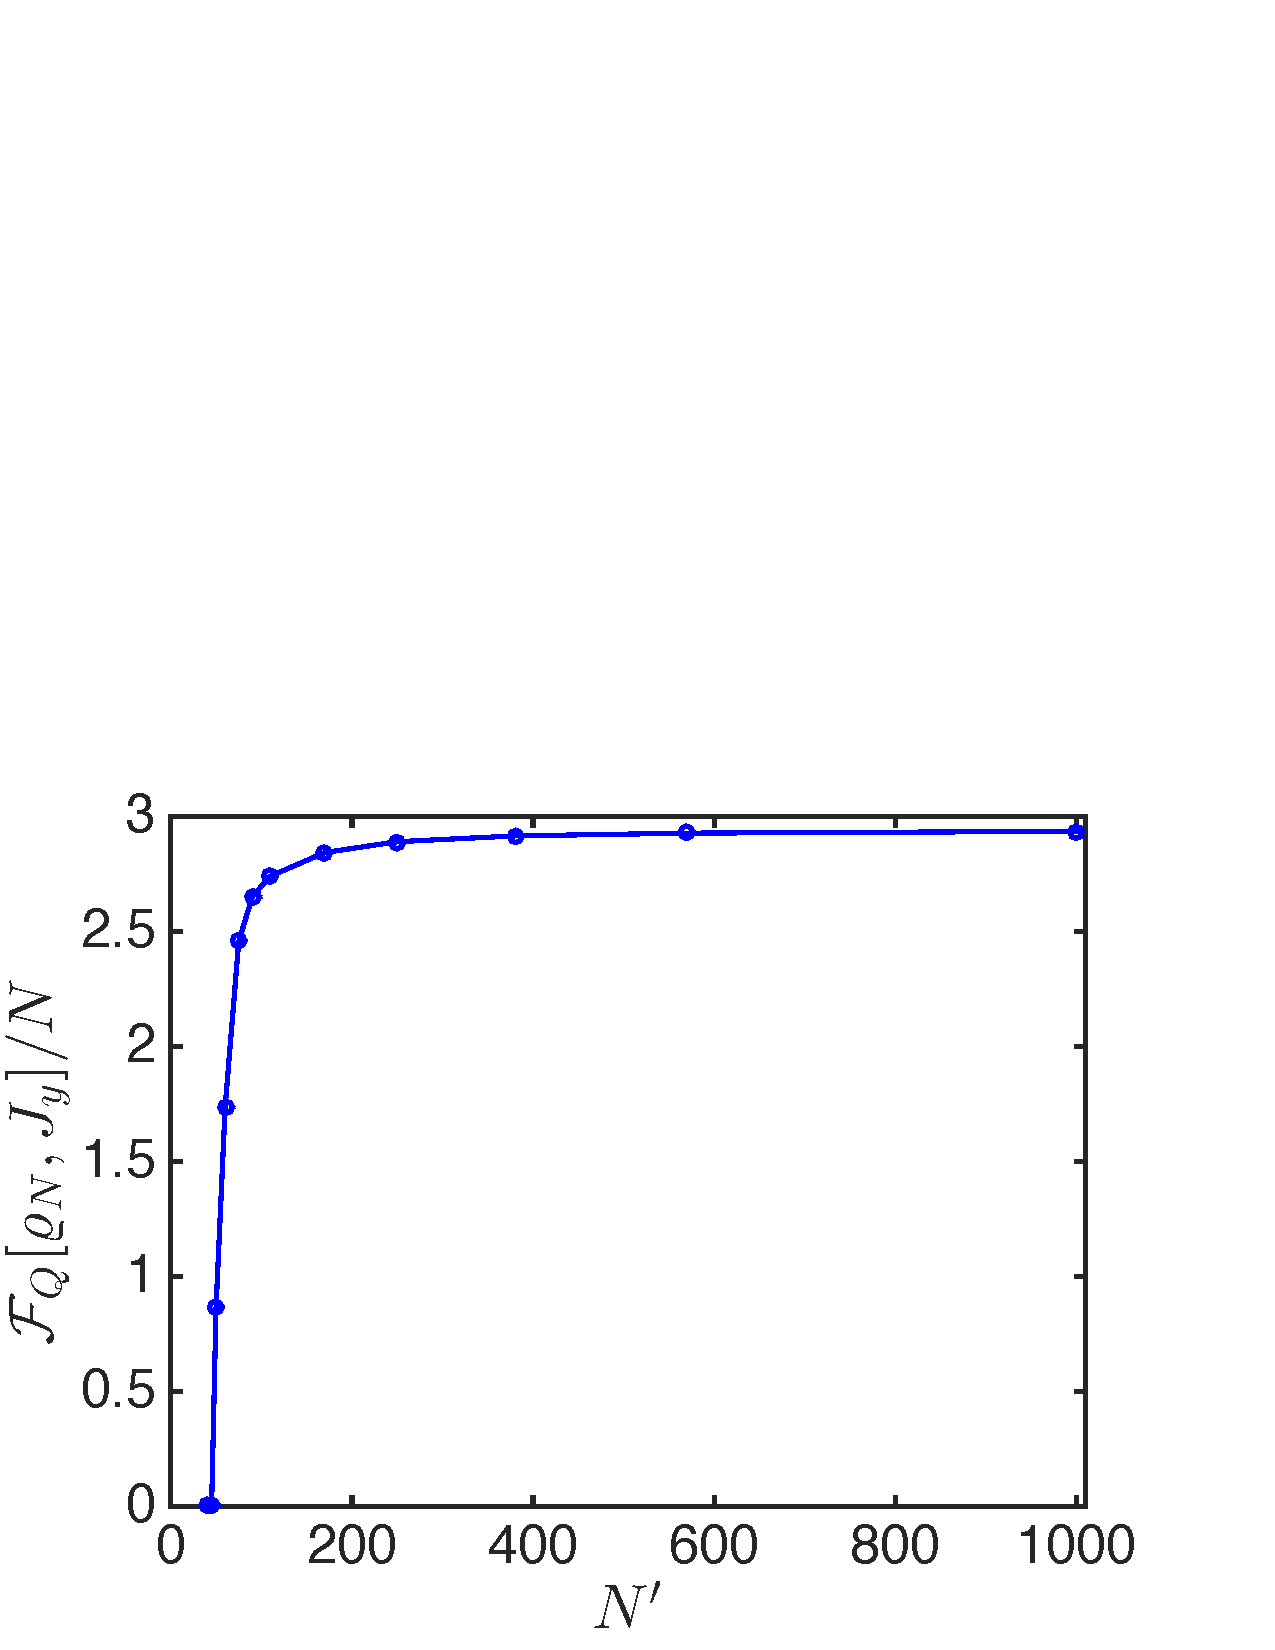
\includegraphics[height=120px]{img/asymptoticapproach-dicke.pdf}
			\end{figure}
			Similarly to spin-squeezed states, the bound \emph{\color{blue}converges quickly}.

			\citate{\textbf{I.A.}, M. Kleinmann, O. G\"une \& G. T\'oth, arXiv:1511.05203}
		\end{frame}

\section{Conclusion and outlook}

	\begin{frame}
		\frametitle{Conclusion and Outlook}
		\begin{enumerate}
			\item<1-> We prove that for realistic cases \emph{\color{blue}the optimisation is feasible}.
			\vspace{5px}
			\item<2-> We used \emph{\color{blue}our approach to verify} that the P-S bound is tight.
			\vspace{5px}
			\item<3-> We have shown that the lower bounds can be \emph{\color{blue}improved with few extra considerations}.
			\vspace{5px}
			\item<4-> For large systems the \emph{\color{blue}optimisation method can be complemented} with scaling considerations.
			\vspace{5px}
			\item<5-> The \emph{\color{blue}method very versatile} and it can be used in many other situations.
		\end{enumerate}

	\end{frame}


\setbeamertemplate{navigation symbols}{}{%

}
\section*{}
	\begin{frame}
		\emph{\LARGE Thank you for your attention!}

		\vspace{15px}
		Preprint $\rightarrow$ arXiv:1511.05203

		\vspace{10px}
		Groups' home pages

		\hspace{15px} $\rightarrow$ \emph{\color{blue} https://sites.google.com/site/gedentqopt}

		\hspace{15px} $\rightarrow$ \emph{\color{blue} http://www.physik.uni-siegen.de/tqo/}
		\vspace{10px}

		\begin{figure}
			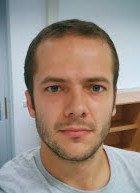
\includegraphics[height=60px]{img/authors/iagoba.jpg}
			\hspace{10px}
			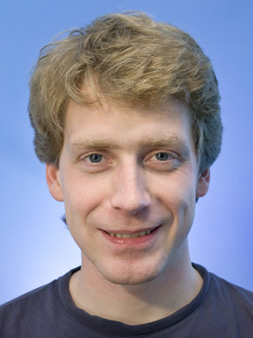
\includegraphics[height=60px]{img/authors/matthias.jpg}
			\hspace{10px}
			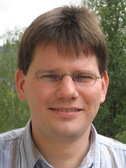
\includegraphics[height=60px]{img/authors/otfried.jpg}
			\hspace{10px}
			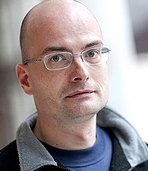
\includegraphics[height=60px]{img/authors/geza.jpg}
		\end{figure}
		\vspace{-25px}

		\begin{center}
			iagoba \hspace{16px}
			matthias \hspace{16px}
			otfried \hspace{30px}
			g\'eza {\color{white}>}
		\end{center}
	\end{frame}

\end{document}
